\subsection{Experimento sintético de ajuste de timing}
\label{sec:timing-sintetico}

Para quantificar esse efeito, considera-se uma série de um pulsar com
$N=256$ observações em $T=4,5$ anos. Comparam-se datas regulares
$t_j=jT/N$ e datas perturbadas por deslocamentos uniformes de até
$0,2T/N$ em cada sentido. O processo temporal combina ruído branco de
100 ns e vinte modos Fourier vermelhos, com variância proporcional a
$k^{-13/3}$ e variância do primeiro coeficiente complexo de
$10^4$ ns$^2$. Esse exemplo isola o ajuste de timing; a população de
pulsares da seção seguinte conserva seu desenho periódico original.

Definem-se três ajustes de mínimos quadrados com pesos iguais: nenhum
ajuste; remoção de constante, termo linear e termo quadrático; e esses
três termos acrescidos de seno e cosseno com período de um ano. Os
termos polinomiais representam fase, frequência de rotação e sua
derivada, enquanto os anuais ilustram o ajuste astrométrico. Se $U_M$
é uma base ortonormal das colunas de $M$, o projetor residual é
\begin{equation}
 R_M=I-U_MU_M^{\mathsf T},\qquad
 \widehat q=D R_M\boldsymbol d,
 \qquad D_{kj}=N^{-1/2}e^{-2\pi i k t_j/T},\quad k=1,\ldots,8.
\end{equation}
A covariância e a pseudocovariância previstas são
$C=D R_M K R_M D^\dagger$ e $P=D R_M K R_M D^{\mathsf T}$.
Um termo determinístico $M\delta\xi$ foi injetado nas séries e removido
por ajuste independente em cada realização. A mudança de covariância
decorre da projeção do processo estocástico, e não da adição de uma
média determinística.

Na grade regular sem ajuste, $C$ é diagonal e $P=0$ à precisão
numérica, recuperando o controle Fourier próprio. Após o ajuste
polinomial, surgem correlações entre frequências e pseudocovariância,
mesmo sem irregularidade nas datas. A inclusão dos termos anuais
amplia esse efeito. Para comparar escalas distintas, usam-se
$\rho_{kl}=C_{kl}/\sqrt{C_{kk}C_{ll}}$ e
$\eta_{kl}=P_{kl}/\sqrt{C_{kk}C_{ll}}$.

\begin{table}[htbp]
\centering
\caption{Dependência entre os oito canais Fourier após o ajuste de
timing. A KL compara a distribuição real conjunta com a aproximação
complexa própria de canais independentes, preservando as variâncias
marginais.}
\label{tab:timing-projecao}
\begin{tabular}{llrrr}
\toprule
Amostragem & Ajuste & $\max_{k\ne l}|\rho_{kl}|$ & $\max|\eta_{kl}|$ & KL (nat)\\
\midrule
Regular & Nenhum & $<10^{-10}$ & $<10^{-10}$ & $<10^{-10}$\\
Regular & Rotação & 0,614 & 0,734 & 3,714\\
Regular & Rotação + anual & 0,706 & 0,746 & 11,218\\
Irregular & Nenhum & 0,002 & 0,005 & $9,28\times10^{-5}$\\
Irregular & Rotação & 0,614 & 0,734 & 3,692\\
Irregular & Rotação + anual & 0,706 & 0,746 & 11,158\\
\bottomrule
\end{tabular}

\end{table}

As previsões foram confrontadas com 20.000 realizações independentes
por esquema de amostragem, reutilizadas entre os três ajustes.
Os coeficientes do modelo de timing foram estimados por mínimos
quadrados em cada série, separadamente da construção matricial do
projetor. As covariâncias reais empíricas concordaram com as previstas:
o maior desvio foi 3,06 erros padrão de uma entrada, calculados pelos
momentos de Wishart para covariâncias gaussianas. O limiar simultâneo
predefinido, pela aproximação normal desses estimadores e correção de
Bonferroni para 816 entradas, foi de 4,85 erros padrão.

\begin{figure}[htbp]
\centering
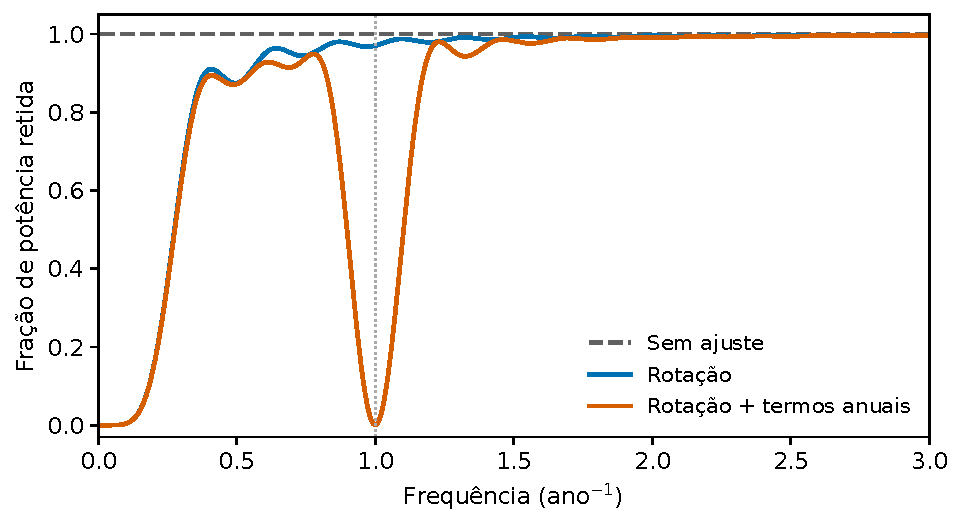
\includegraphics[width=\textwidth]{../figures/timing/transferencia.pdf}
\caption{Potência de uma senoide retida nos resíduos, em função da
frequência, com média sobre a fase inicial. O ajuste polinomial suprime
baixas frequências; os termos anuais removem a componente de período
de um ano. As curvas usam datas regulares.}
\label{fig:timing-transferencia}
\end{figure}

A Figura~\ref{fig:timing-transferencia} mostra a fração de energia
temporal retida após projetar uma senoide. A depressão anual é
consequência direta de incluir essa senoide na base ajustada.
Essa fração descreve a remoção de um sinal monocromático; a covariância
Fourier de um espectro amplo inclui também a mistura entre frequências.

\begin{figure}[htbp]
\centering
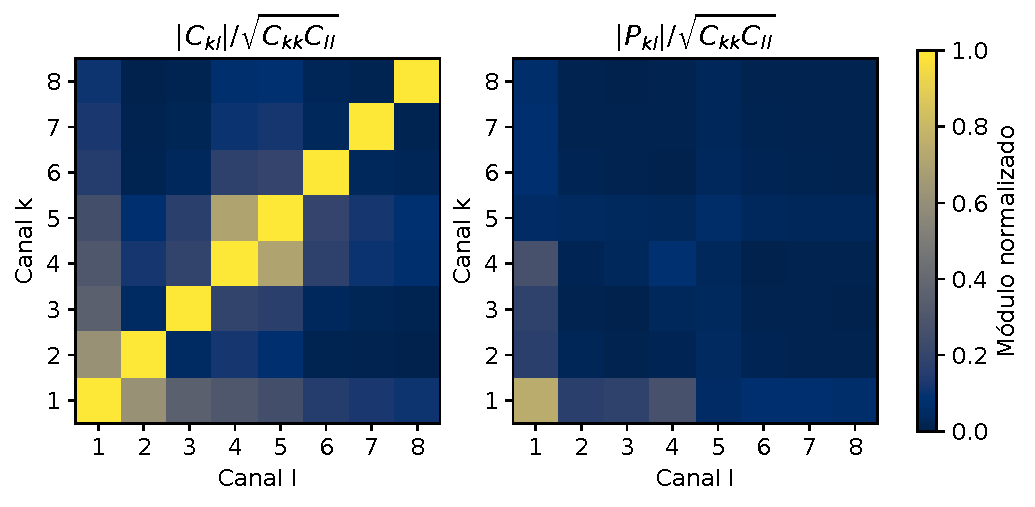
\includegraphics[width=\textwidth]{../figures/timing/covariancias.pdf}
\caption{Módulos da correlação entre canais (esquerda) e da
pseudocovariância normalizada (direita), para cadência regular com
ajuste de rotação e termos anuais. Os elementos fora da diagonal à
esquerda e os elementos não nulos à direita evidenciam a quebra das
hipóteses de independência e propriedade complexa.}
\label{fig:timing-covariancias}
\end{figure}

O efeito também pode ser expresso pela diferença entre distribuições
gaussianas. Seja $K_R$ a covariância real exata dos dezesseis
coeficientes reais e imaginários e $K_A$ a da aproximação considerada.
Para médias nulas,
\begin{equation}
 D_{\rm KL}(\mathcal N_{K_R}\Vert\mathcal N_{K_A})=
 \frac12\left[\operatorname{tr}(K_A^{-1}K_R)-16+
 \log\frac{\det K_A}{\det K_R}\right].
\end{equation}
Na grade regular com ajuste anual, conservar $C$ inteiro, mas impor
$P=0$, já produz 6,31 nat. Impor também independência entre canais
eleva a divergência para 11,22 nat. Trata-se de discrepância entre
distribuições de dados, distinta da informação posterior--priori
sobre a massa. Todas as covariâncias reais deste teste têm posto 16.

Esse experimento demonstra que a hipótese de coeficientes próprios
independentes exige verificação após o ajuste de timing. A aplicação
à massa do gráviton requer incorporar essa projeção à covariância
multípulsar, juntamente com o modelo de ruído e as datas observacionais.
